\documentclass[11pt,a4paper,oneside]{article}

\usepackage[left=3.5cm,right=2.5cm,top=3cm,bottom=4cm,headsep=7ex,footskip=1.5cm]{geometry}
\usepackage[german]{babel}
\usepackage[utf8]{inputenc}
\usepackage{graphicx}
\usepackage{float}
\usepackage{wrapfig}
\usepackage{listings}
\usepackage{caption}
\usepackage{matlab-prettifier}
\usepackage[T1]{fontenc}
\usepackage[utf8]{inputenc} 
\usepackage{tabularx}
\usepackage{booktabs}
\usepackage[straightvoltages]{circuitikz}

%\usepackage[backend=biber,style=alphabetic]{biblatex}

\usepackage{textgreek}


%\setlanguage{\english}

\newcommand{\relpath}{./}

% This is more or less the "Main" of our latex document. All the files are put together here.
% Adapt the variables for your case accordingly

\def\titlelength{0}
\def\type{Labor Report}
\def\lecture{Titel der LV}
\def\codeStudydegreeyear{MGST-B-2-MR-MSR-ILV}
\def\subtitle{Aufgabe 1}
\def\semester{Wintersemester  2024/2025}
\def\student{Max Mustermann\newline Maria Musterfrau}
\def\lecturer{Dr. Gerda Strutzenberger\newline Prof.Dr.Dipl Daniel Sieber\newline Prof Yeongmi Kim\newline Prof Bernhard Hollaus}

\usepackage{ifthen}
\newboolean{skript}
\setboolean{skript}{true}

% layout
\usepackage{fancyhdr}
\setlength{\headheight}{14pt}
\usepackage{wallpaper}
\usepackage{float}
\usepackage[colorlinks=true,urlcolor=black,linkcolor=black]{hyperref}  
\hypersetup{
	pdftitle= {Lab1},
	pdfauthor={xxx},
	pdfsubject = {xxx},
}
\hypersetup{%
  citecolor=black
}

\ifthenelse{\boolean{skript}}{
	% no page numbering on part page
	\makeatletter
	\renewcommand\part{%
	  \if@openright
		\cleardoublepage
	  \else
		\clearpage
	  \fi
	  \thispagestyle{empty}%
	  \if@twocolumn
		\onecolumn
		\@tempswatrue
	  \else
		\@tempswafalse
	  \fi
	  \null\vfil
	  \secdef\@part\@spart}
	\makeatother
}{}

\parindent0pt

% graphics
\usepackage{epstopdf}
\usepackage{pst-all}
\usepackage{float}
%\usepackage[dvips,clip]{graphicx}
\usepackage{graphicx}
\usepackage{exscale,relsize}
\usepackage{psfrag}
\usepackage[font={small,it},format=hang]{caption}	% will apply to all captions
\usepackage[font={small,it},format=hang]{subcaption} % will apply to all subcaptions
\usepackage[percent]{overpic}
\usepackage[most]{tcolorbox}
\newtcolorbox{mytextbox}[1][]{%
  sharp corners,
  enhanced,
  colback=red,
  height=3.7 cm,
  attach title to upper,
  #1
}

\newcommand\blankpage{
\null
\thispagestyle{empty}
\addtocounter{page}{-1}
\newpage}

%\usepackage[duplicate]{chapterbib.bib}
%\usepackage[refsection=part,backend=biber]{biblatex}
\usepackage{minitoc}

% equations
\usepackage{amsmath}
\usepackage{amssymb}
\usepackage{amsthm}
\usepackage{mathrsfs}
\usepackage{amsxtra}
\usepackage{xfrac}
\usepackage{bbding}

% including code
\usepackage{verbatim}
\usepackage{moreverb}
\usepackage{url}

% layout stuff
\renewcommand{\labelitemi}{-}

% headline
\pagestyle{fancy}
%\lhead{\nouppercase{\leftmark}}
\rhead{\thepage}
\cfoot{}
\renewcommand{\headrulewidth}{0.4pt}

% footline  
\lfoot{{\it\footnotesize \lecture}}
\rfoot{{\it\footnotesize \semester}}
\renewcommand{\footrulewidth}{0.0pt}

% \ifthenelse{\boolean{skript}}{
	% \renewcommand{\chaptermark}[1]{\markboth{\thechapter.\ #1}{}}
% }{}

\usepackage{listings} 
% mcode package for MATLAB code highlighting
%\usepackage{mcode}
%\lstloadlanguages{figure}

% Setup the listings settings
\lstset{
    frame=leftline,
    rulecolor=\color{gray},
	escapeinside={(*@}{@*)},
	language=C,
	aboveskip=3mm,
	belowskip=3mm,
	showstringspaces=false,
	columns=flexible,
	basicstyle={\fontfamily{pxtt}\selectfont\footnotesize},
	numbers=left,
	stepnumber=2,
	numberstyle=\tiny\color{gray},
	numberblanklines=true,
	breaklines=true,
	breakatwhitespace=true,
	tabsize=2,
	captionpos=b,
}

% Monochrome style
\lstdefinestyle{bw}{
    backgroundcolor=\color{white},
    keywordstyle=\bfseries,
	commentstyle=\itshape,
	stringstyle=\slshape,
}

% RAPID language definition
\lstdefinelanguage[]{RAPID}%
{
	keywords={LOCAL,VAR,MODULE,FUNC,ENDFUNC,RETURN,TRUE,FALSE,ENDMODULE,NOT,PROC,ENDPROC,IF,ELSE,ENDIF,THEN,\\PERS, FOR, FROM, TO, DO, ENDFOR, MOD},
	otherkeywords={...},
	comment=[l]{!},%
	morecomment=[s]{/*}{*/},%
	string=[b]{"},%
	alsoletter={\\}
}[keywords,comments,strings]%

% XML language definition
\lstdefinelanguage{XML}
{
	morestring=[s]{"}{"},
	morecomment=[s]{<!--}{-->},
	%stringstyle=\color{black},
	%identifierstyle=\color{blue},
	%keywordstyle=\color{cyan},
	morekeywords={xmlns,version,type}% list your attributes here
}

% Old style
% ansys style 
%\lstloadlanguages{fig.}
%\lstset{
%language=ansys,
%numbers=left, 
%numberstyle=\scriptsize, 
%stepnumber=1, 
%keywordstyle=\color{blue},
%numbersep=5pt,
%frame=single,
%backgroundcolor=\color[rgb]{0.85, 0.85, 0.85},
%frameround=tttt,
%basicstyle=\ttfamily\scriptsize,
%breaklines=true,
%framextopmargin=50pt,
%frame=bottomline, 
%}

\renewcommand{\lstlistlistingname}{List of Code}

\input{"sub/_definitions/definitions_new_commands.tex"}

%\addbibresource{literature.bib}

% für Deckblatt von A. Mehrle
\newboolean{english}
%\setboolean{english}{true}		% auskommentieren fuer deutsche Version
\newboolean{student}
\setboolean{student}{true}		% auskommentieren fuer Lektorenversion 

% Use of Subfiles
\usepackage{subfiles}

% Units
% \usepackage{units}

% Counter for continuous roman counting
\newcounter{romancount}

% Acronyms
\usepackage[printonlyused]{acronym}
\newcommand{\listofacronyms}{\input{"sub/acronyms.tex"}}

% for using \FloatBarrier
% option "section" so that floats to not cross section border by default
\usepackage[section]{placeins}

% Including pdf pages
\usepackage[final]{pdfpages}

% LoX as sections (was chapter)
\makeatletter
\renewcommand\listoffigures{%
  \section*{\listfigurename}%
  \@mkboth{\MakeUppercase\listfigurename}{\MakeUppercase\listfigurename}%
  \@starttoc{lof}%
}
\renewcommand\listoftables{%
  \section*{\listtablename}%
  \@mkboth{\MakeUppercase\listtablename}{\MakeUppercase\listtablename}%
  \@starttoc{lot}%
}
\renewcommand\lstlistoflistings{%
  \section*{\lstlistlistingname}%
  \@mkboth{\MakeUppercase\lstlistlistingname}{\MakeUppercase\lstlistlistingname}%
  \@starttoc{lol}%
}
\makeatother

% Blindtext
\usepackage{blindtext}
% graphics paths compiling from main and compiling from subfile
\graphicspath{{sub/_fig.s/}{.._/fig.s/}}

\begin{document}
\pagenumbering{Roman}
%%%%%%%%%%%%%%%%%%%%%%%%%%%%%%%%%%%%%%%%%%%%%%%%%%%%%%%%%%%%%%%%%%%%%%%%%%%
\begin{titlepage}


\thispagestyle{empty}
\enlargethispage{5cm}

% set MCI logos as background
\ThisULCornerWallPaper{}{sub/_definitions/header}
%
\vspace*{-3.4cm}
{\color{white}\scriptsize\sffamily\bfseries\hspace*{7.42cm}\vspace*{-1.5ex}DIE UNTERNEHMERISCHE HOCHSCHULE\textsuperscript{\textregistered}\\\hspace*{7.42cm}\vspace*{-1ex}MCI MANAGEMENT CENTER INNSBRUCK\\}
{\color{white}\tiny\sffamily\bfseries\hspace*{9.1cm}\vspace*{-2ex}A-6020 Innsbruck, Universit\"atsstra\ss e 15\\\hspace*{9.1cm}+43 512 2070 0, office@mci.edu, www.mci.edu}
% -------- only change entries beginning here ----------------------------
%
% enter the study (Studienrichtung)
% z.B. \def\study{Mechatronik - Maschinenbau}
\ifthenelse{\boolean{english}}{\def\study{Bachelor Medical, Health and Sports Engineering}}{\def\study{Bachelor Medizin-, Gesundheits- und Sporttechnologie}}
%
%
% enter the name of the institute
% z.B. \def\institute{Management Center Innsbruck}
\def\institute{\includegraphics[width=5cm]{sub/_definitions/MCI_4C}}
%
% enter date
\def\date{\today}

\def\diplskip{\ifnum\titlelength>2\medskip\else\bigskip\fi}
\def\varskip{\ifcase\titlelength\bigskip\bigskip\bigskip\or\bigskip\bigskip\or\bigskip\else\smallskip\fi}
\def\ifundefined#1{\expandafter\ifx\csname#1\endcsname\relax}
\unitlength 1cm

\begin{picture}(0,0)

%\put(-.97,-4.2){\begin{minipage}[t]{17cm}
\put(-.97,-4.2){\begin{minipage}[t]{\textwidth} %CAS
\begin{center}
\Large\textsc{\type}
\bigskip\par
\LARGE \textbf{\lecture}
\smallskip\par
\LARGE \textbf{\codeStudydegreeyear}
\bigskip\par
\large \textbf{\subtitle}
\bigskip\par
% Lecturer: Alexander Walder, B.Sc.
\varskip\bigskip\par
\Large \textsc{\semester}
\varskip\bigskip\par
\normalsize \ifthenelse{\boolean{english}}{study program}{Studiengang} 
\bigskip\par
\Large \textsc{\study}
\end{center}
\vspace*{2mm}
\bigskip\bigskip\par
\vspace*{6mm}
\begin{minipage}[t]{6.9cm}
    \begin{flushleft} \large
    \normalsize \ifthenelse{\boolean{english}}{Authors}{Verfasser}:
    \smallskip\par
    \large\textsl{\student}
    \bigskip\par
    \normalsize \ifthenelse{\boolean{english}}{Lecturer}{LV-Leiter}:
    \smallskip\par
    \large\textsl{\lecturer}
    \end{flushleft}
\end{minipage}
\diplskip\bigskip\par
\diplskip\bigskip\par
\normalsize \ifthenelse{\boolean{english}}{last update}{letzte Aktualisierung}: \date
\diplskip\par
\diplskip\par
\bigskip
\bigskip\bigskip
\ifnum\titlelength>2\bigskip\bigskip\else\bigskip\bigskip\medskip\fi
\par
\normalsize {\sl \institute}
\end{minipage}}
\end{picture}
\end{titlepage}

\newpage
%%%%%%%%%%%%%%%%%%%%%%%%%%%%%%%%%%%%%%%%%%%%%%%%%%%%%%%%%%%%%%%%%%%%%%%%%%%
%\blankpage
\setcounter{page}{2}
\tableofcontents
\vspace{2cm}
%\clearpage
	\newpage
	%% Remember roman page count for continuing in appendix
	\setcounter{romancount}{\value{page}}
    	\setcounter{page}{1}

	\pagenumbering{arabic}
	

	\section{Einleitung und Zielsetzung}
In diesem Labor soll die Aufzeichnung und Verarbeitung von EMG-Signalen
(EMG: Elektromyographie) erlernt werden. Dafür werden EMG-Signale von
verschieden intensiven Muskelaktivitäten aufgenommen und anschliessend mit
verschiedenen Methoden der Signalverarbeitung analysiert. Ziel ist es, die
Unterschiede der Signale zu erkennen und zu quantifizieren.
Die EMG-Signale werden mit Hilfe von Oberflächenelektroden erfasst, die auf der
Hautoberfläche über dem Muskel angebracht werden. Die Signale werden dann
verstärkt, gefiltert und digitalisiert, um sie für die weitere Analyse
vorzubereiten. % have a look inside the tex files regarding  the sections. Here they are only added one after another
    \clearpage  %Weil die section davor mit einer Floating tabelle endet, funktioniert der \newpage Befehl nicht richtig
	\section{Vorbereitende Arbeiten}
Es wurden im Rahmen dieser Laboreinheit folgende Komponenten und Software verwendet:

\begin{table}[ht]
    \centering
    \begin{tabularx}{\textwidth}{l l X}
        \hline
        Typ & Modell & Verwendung \\
        \hline
        Microcontroller & Sparkfun RedBoard & Zur Erfassung der Sensordaten und Übertragung an den Computer \\
        Sensor & EMG/EKG Sensor & Zur Messung der elektrischen Signale des Herzens \\
        Software & Arduino IDE 1.8.19 & Zur Programmierung des Arduino Mikrocontrollers \\
        Software & Python 3.9 (Jupyter Notebook / VS Code) & Zur Verarbeitung, Aufzeichnung und Visualisierung der Sensordaten \\
        USB-Kabel & Standard USB A to B Kabel & Zur Verbindung des Arduino mit dem Computer mittels COM4 \\
        3 Jumper Kabel & Standard Jumper Kabel & Zur Verbindung des EMG-Sensors mit dem Arduino \\
        Elektroden & Standard EKG-Elektroden & Zur Ableitung der elektrischen Signale des Herzens \\
        \hline
    \end{tabularx}
    \caption[Verwendete Komponenten und Software]{Die im Rahmen der Laboreinheit verwendeten Komponenten und Software}
    \label{tab:verwendete_komponenten}
\end{table}


Das Skript zum Aufzeichen und Speichern der Sensor Rawdaten wurde von Team der Lehrerenden bereitgestellt und konnte ohne große Anpassungen verwendet werden.
--> hier vllt Link zu Datei oder Repository einfügen <--
Auch für die Visualisierung der Daten wurde ein Skript zur Verfügung gestellt, welches unter Anderem auf Grund von Artefakten leicht auf unseren spezifischen Fall angepasst werden musste.
--> hier vllt Link zu Datei oder Repository einfügen <--


\begin{figure}[htbp]
    \centering
    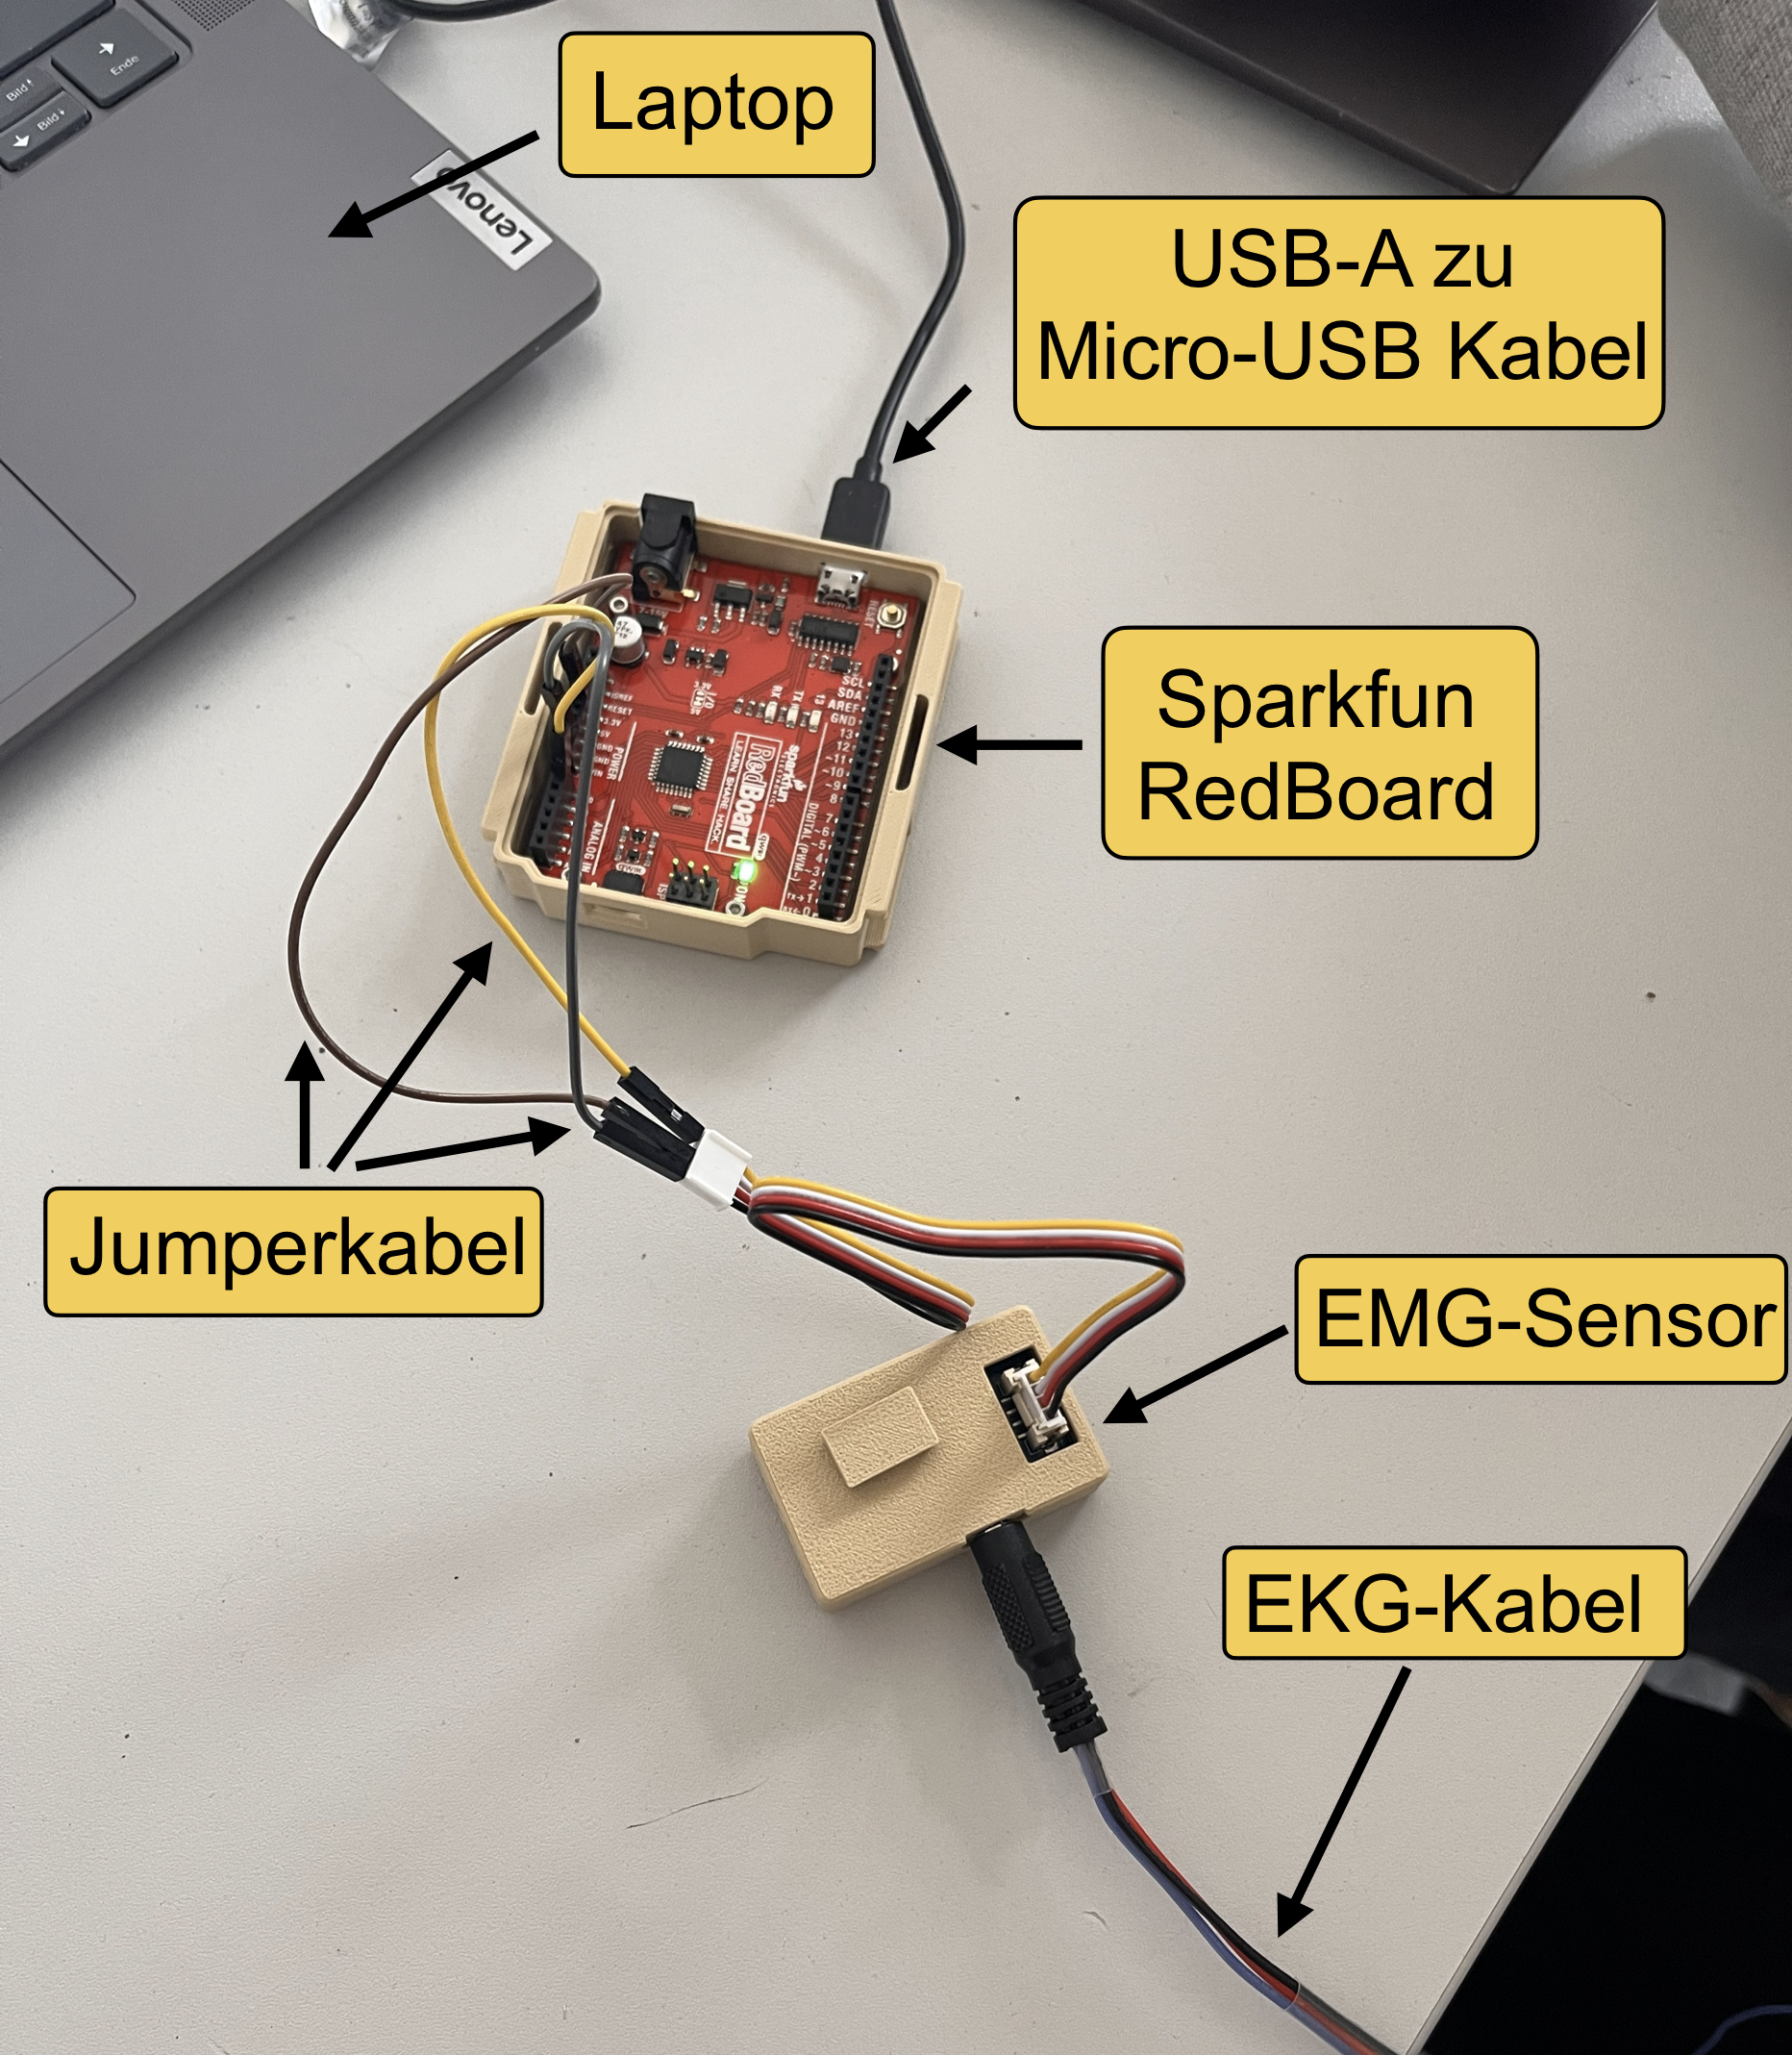
\includegraphics[width=0.7\textwidth]{figures/versuchsaufbau.png}
    \caption{Verbindung des EMG/EKG Sensors mit dem Sparkfun RedBoard Mikrocontroller}
    \label{fig:versuchsaufbau}
\end{figure}

Vor Beginn der eigentlichen Messungen musste der in Tabelle \ref{tab:verwendete_komponenten} erwähnte Sparkfun RedBoard Mikrocontroller über die drei Jumper Kabel mit dem EMG/EKG Sensor verbunden werden wie in Abbildung \ref{fig:versuchsaufbau} zu erkennen ist.
Die Elektroden des Sensors wurden anschließend an den Probanden / die Probanden angebracht. Die drei Elektroden sind am Manubrium, am linken V6 Ableitpunkt und am C7 der Halswirbelsäule angeklebt worden.\\

\begin{figure}[htbp]
    \centering
    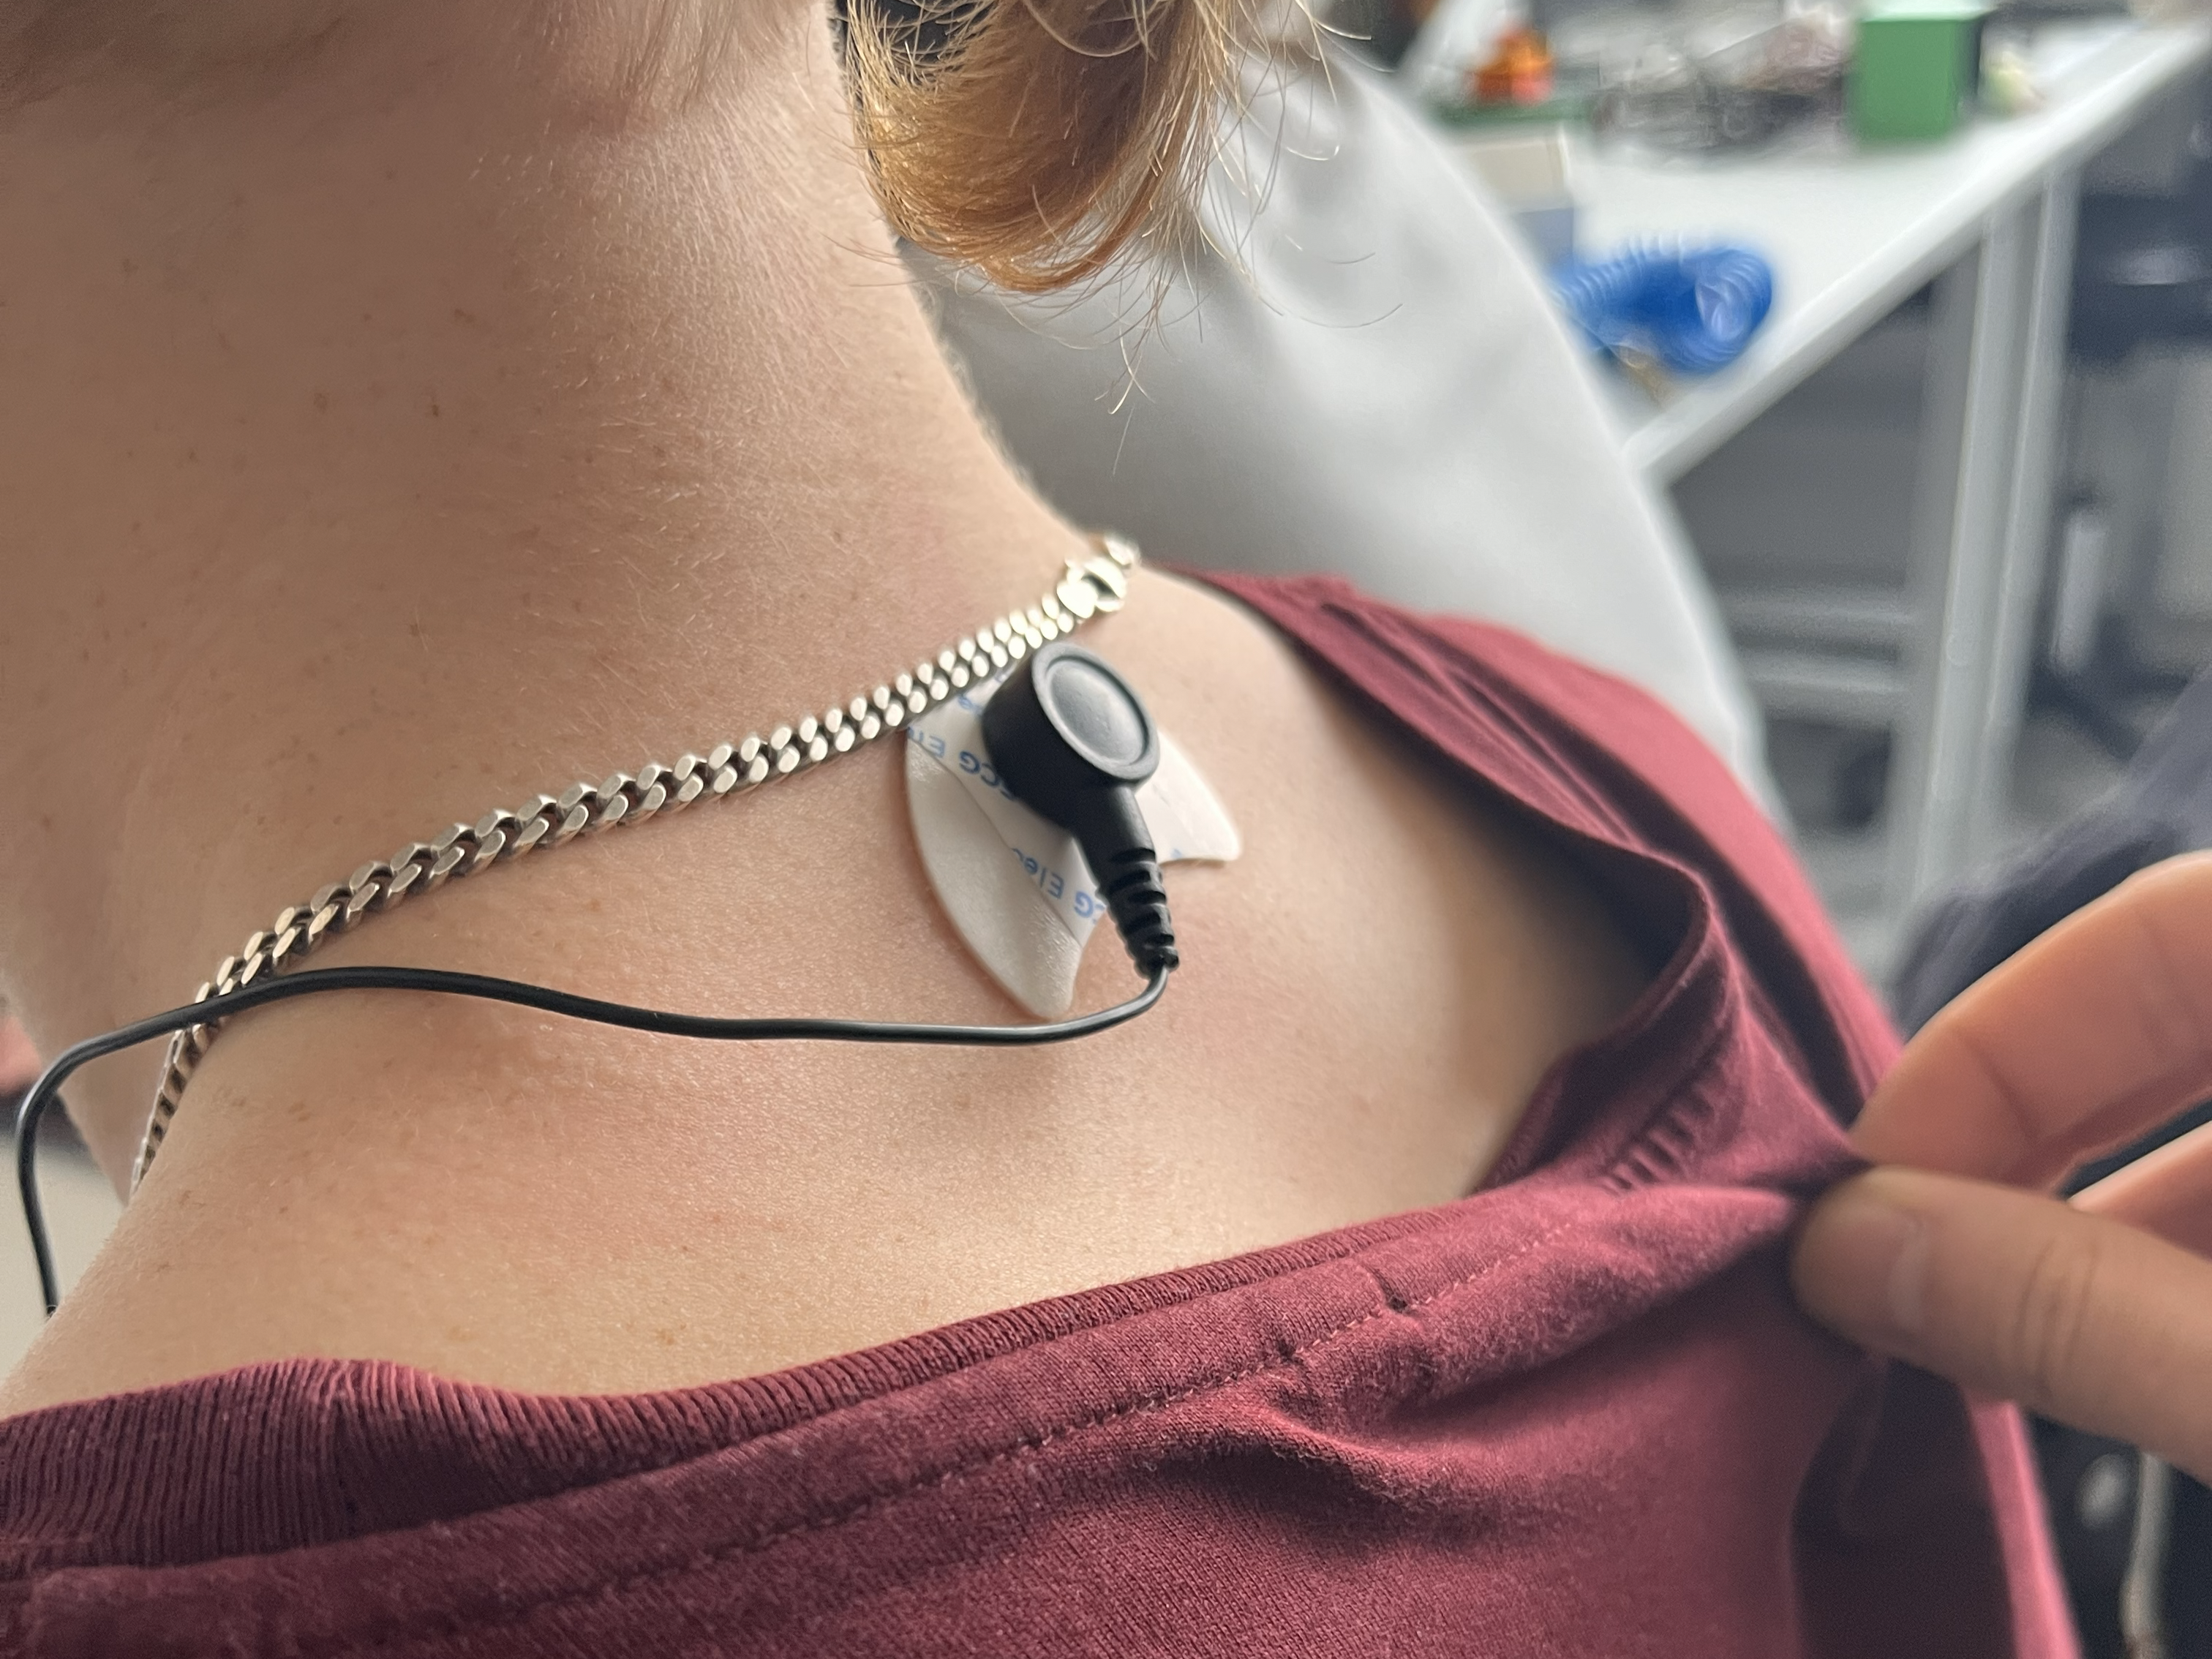
\includegraphics[width=0.7\textwidth]{figures/GNDelectrode_C7.png}
    \caption{Position der Ground-Elektrode auf dem C7 der Halswirbelsäule}
    \label{fig:gnd_electrode_c7}
\end{figure}

in der Abbildung \ref{fig:gnd_electrode_c7} ist die Position der Ground-Elektrode auf dem C7 der Halswirbelsäule zu sehen.

\begin{figure}[htbp]
    \centering
    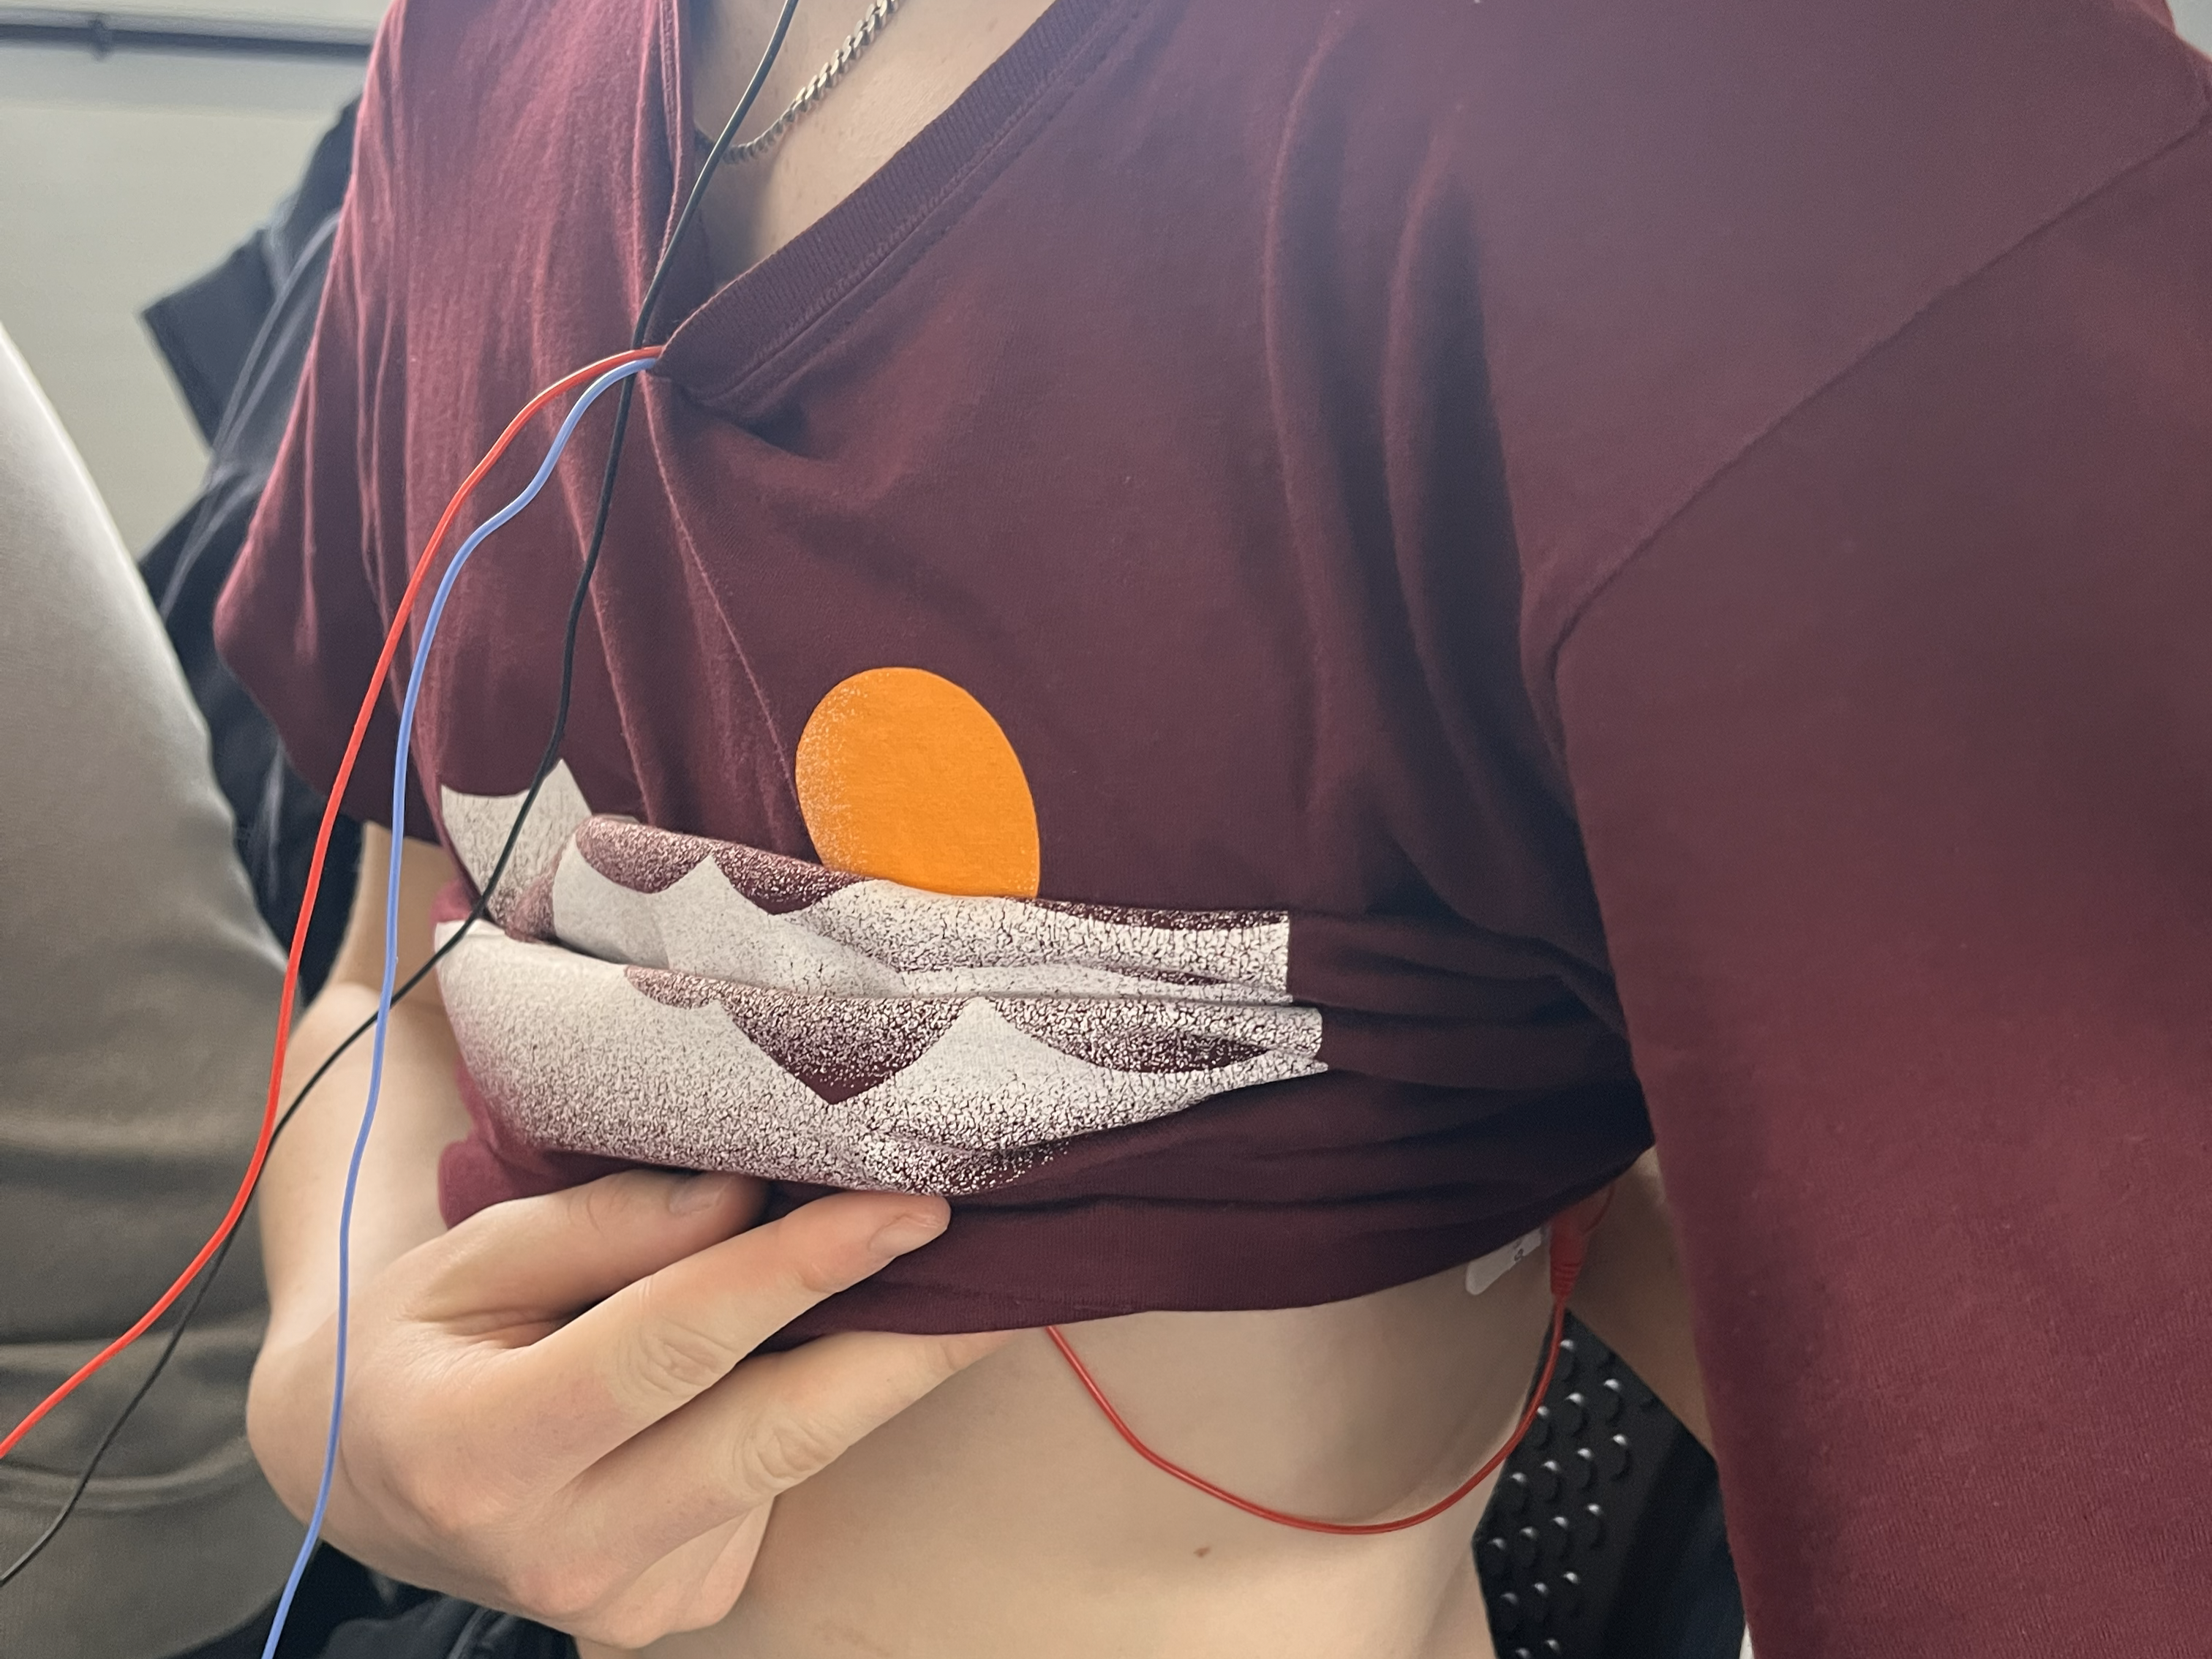
\includegraphics[width=0.7\textwidth]{figures/Manubrium_and_6rip.png}
    \caption{Position der V6-Elektrode auf dem linken V6 Ableitpunkt und der Spannungsquelle auf dem Manubrium}
    \label{fig:v6_electrode_left_and_manubrium}
\end{figure}

In der Abbildung \ref{fig:v6_electrode_left_and_manubrium} ist die Position der V6-Elektrode auf dem linken V6 Ableitpunkt - rotes Kabel - sowie der Spannungsquelle auf dem Manubrium - blaues Kabel - zu sehen.
    \newpage
	\section{Versuchsaufbau und Durchführung}
\subsection{Aufgabe 1: Diagramme der Komponenten}

\subsection{Aufgabe 2: Daten im Seriellen Plotter}
Im seriellen Plotter wurden die Rohdaten des EKG-Signals visualisiert. Dabei konnte beobachtet werden,
dass, sobald der Laptop über ein Netzteil mit Strom versorgt wurde, starke Störungen in Form von Noise im Signal auftraten.
Der Noise hat eine Frequenz von circa 50 Hz, weshalb davon auszugehen ist, dass es sich um Netzbrummen handelt.
Das Netzbrummen wurde durch die Verwendung des Laptops im Akkubetrieb vermieden. Alternativ wäre eine Filterung des Signals mit Tiefpassfiltern möglich gewesen.

\subsection{Aufgabe 3: Experiment in Ruhe}

\subsection{Aufgabe 4: Beschreibung und Erklärung des Ruhe-EKG Codes}
\subsubsection{Arduino Code}
Das bereitgestellte Skript Lab2Code1 \cite{Lab2Code1.ino} wurde verwendet, um die Rohdaten des EKG-Signals zu erfassen und über die serielle Schnittstelle an den Computer zu übertragen.
Von dort aus wurden die Daten im nachfolgenden Skript serialRead \cite{serialRead.ipynb} eingelesen und gespeichert, wie in Abschnitt \ref{sssec:PythonCode} beschrieben wird.
Der Code initialisiert die serielle Kommunikation mit einer Baudrate von 500000 und liest kontinuierlich die analogen Werte vom EKG-Sensor ein.
Dieser Wert wird dann nur an die Console weitergegeben, wenn eine Zeit von 1000 Millisekunden vergangen ist.
\subsubsection{Python Code}
\label{sssec:PythonCode}
Der Code serialRead \cite{serialRead.ipynb} wurde ebenfalls bereitgestellt. 
In diesem Skript können die serielle Schnittstelle, die Baudrate und die Dauer der Aufnahme sowie der Name des Outputdokuments als Variablen gesetzt werden.
Die Funktion sampling() öffnet die serielle Schnittstelle und das Outputdkoument und liest dann die Daten für die angegebene Dauer ein.
Die eingelesenen Daten werden in eine Liste gespeichert und anschließend in das Outputdokument geschrieben.
Danach werden Informationen zur gemittelten Samplingrate über die gesamte Aufnahmezeit, totale Anzahl an Samples und vergangener Zeit sowie der Speicherbestätigung ausgegeben.
Die Funktion returned den Wert der errechneten Sampling Rate.
Im zweiten Teil des Codes werden die Daten aus dem Outputdokument eingelesen und in einem Plot visualisiert, um direkt die Qualität der Aufnahme beurteilen zu können.

\subsection{Aufgabe 5: Fünf-Sekunden-Plot der Ruhe-EKGs}

\subsection{Aufgabe 6: Errechnete Daten der Ruhe-EKGs}

\subsection{Aufgabe 7: Einordnung der Daten im Kontext derer der Mitstudierenden}
In den Histogrammen zeigt sich, dass die mittlere Herzfrequenz bei Frauen und Männern ähnlich verteilt ist,
wobei beide Geschlechter einen Mittelwert um 63-65 bpm aufweisen. Bei der Herzfrequenzvariabilität ist eine größere Streuung erkennbar,
wobei beide Geschlechter eine breite Verteilung zeigen. Die großen Überlappungen zwischen den Geschlechtern deuten darauf hin,
dass die interindividuelle Variabilität größer ist als geschlechtsspezifische Unterschiede. Mögliche Ursachen für fehlende 
Geschlechtsunterschiede könnten die relativ kleine Stichprobengröße, ähnliche Fitnesslevel der Teilnehmenden oder unterschiedliche 
Messbedingungen sein.

\begin{figure}[htbp]
    \centering
    \includegraphics[width=0.5\textwidth]{figures/Histogramm_Herzfrequenz.png}
    \caption{Histogramm der Herzfrequenzverteilung nach Geschlecht}
    \label{fig:histogram_herzfrequenz}
\end{figure}

Hier kommt dein Text zwischen den beiden Abbildungen...

\begin{figure}[htbp]
    \centering
    \includegraphics[width=0.5\textwidth]{figures/Histogramm_HFV.png}
    \caption{Histogramm der Herzfrequenzvariabilität nach Geschlecht}
    \label{fig:histogram_hfv}
\end{figure}

\subsection{Aufgabe 8: Plott der Herzfrequenz während des Belastungs-EKGs}

\subsection{Aufgabe 9: Ruhephase vor Belastungs-EKG}

\subsection{Aufgabe 10: Erholungsphase nach Belastungs-EKG}

\subsection{Aufgabe 11: Berechnen des metabolischen Energieverbrauchs}

\subsection{Aufgabe 12: Einordnung des Energieverbrauchs und entsprechender Code}
    \newpage
	\section{Ergebnisse und Interpretation}
In diesem Abschnitt werden die Ergebnisse der im Abschnitt Versuchsaufbau und Durchführung beschriebenen Abgabe präsentiert und interpretiert.
\subsection{Abgabe 1}
\subsubsection{Aufgabe 5 (a)}
\begin{figure}[H]
    \centering
    \includegraphics[width=\textwidth]{figures/Lab1_IMU_6Achsentest_Accelerometer.png} 
    \caption{Abgabe 1 - Aufgabe 5 (a)}
    \label{fig:6Achsentest_Accelerometer}
\end{figure}
In Abbildung \ref{fig:6Achsentest_Accelerometer} ist die gemessene Beschleunigung des 6-Achsen-Tests dargestellt.
Die X-, Y- und Z-Achse sind farblich unterschiedlich gekennzeichnet.
Es ist zu erkennen, dass die Beschleunigung in den drei Achsen variiert,
wenn der Sensor in verschiedene Positionen gebracht wird. Dies bestätigt die Funktionsfähigkeit des Beschleunigungssensors.
\newline
Die Farben der entsprechenden Achsen sind wie folgt:
\begin{itemize}
    \item X-Achse: Rot
    \item Y-Achse: Grün
    \item Z-Achse: Blau
\end{itemize}


\begin{figure}[H]
    \centering
    \includegraphics[width=\textwidth]{figures/Lab1_IMU_6Achsentest_Accelerometer_Filtered.png} 
    \caption{Abgabe 1 - Aufgabe 6}
    \label{fig:6Achsentest_Filtered}
\end{figure}
In der obigen Abbildung sind die gleichen Achsen wie in Abbildung \ref{fig:6Achsentest_Accelerometer} verwendet worden.
Der eingesetzte Butterworth-Filter 4. Ordnung hat erreicht, dass die hochfrequenten Anteile des Signals deutlich reduziert wurden.
Dadurch ist das Signal deutlich geglättet und Rauschen wurde entfernt. Da dieser Filter eine hohe Flankensteilheit besitzt,
werden die niederfrequenten Anteile des Signals kaum beeinflusst, was zu einer guten Signalqualität führt.

\subsubsection{Aufgabe 8}
An dieser Stelle muss angemerkt werden, dass die in Abbildung \ref{fig:10s-1Achse_Accelerometer} dargestellten Daten nach dem Anpassen der falsch eingestellten Messparameter aufgezeichnet wurden.
Da wir keine falschen Messwerte aus Aufgabe 8 haben, werden wir uns auf die Beantwortung der Fragen aus den Aufgaben 9 und 12 konzentrieren.

\subsubsection{Aufgabe 9 und 12}

\begin{figure}[H]
    \centering
    \includegraphics[width=0.8\textwidth]{figures/Lab1_10s-1Achse_3Anlauf_Accelerometer.png} 
    \caption{Abgabe 1 - Aufgabe 9}
    \label{fig:10s-1Achse_Accelerometer}
\end{figure}
In Abbildung \ref{fig:10s-1Achse_Accelerometer} ist die gemessene Beschleunigung des 10 Sekunden Tests auf einer Achse dargestellt.
Die X-, Y- und Z-Achse sind farblich wie folgt gekennzeichnet:
\begin{itemize}
    \item X-Achse: Blau
    \item Y-Achse: Orange
    \item Z-Achse: Grün
\end{itemize}
Es ist zu erkennen, dass die meiste Beschleunigung in der X-Achse auftritt, was darauf hinweist, dass die Bewegung hauptsächlich entlang dieser Achse stattgefunden hat.
Die Y- und Z-Achsen zeigen nur geringe Schwankungen, was darauf hindeutet, dass die Bewegung in diesen Richtungen minimal war.
\newline
Folgende Anpassungen mussten vorgenommen werden, um die Messdaten korrekt aufzuzeichnen:

\begin{itemize}
    \item Die Baudrate wurde auf 57600 Baud (Bits per second) geändert, damit die Schnittstelle und der Arduino/Sparkfun die gleiche Baudrate haben.
    \item setscale wurde von 2G auf 8G geändert, um die höheren Beschleunigungswerte korrekt zu erfassen und kein Clipping entsteht (Plateaus).
    \item Die Sample-Rate wurde von 1,56 Hz auf 800 Hz (\texttt{ODR\_1} zu \texttt{ODR\_800}) erhöht, um dem Nyquist-Shannon-Abtasttheorem gerecht zu werden und Aliasing-Effekte zu vermeiden. 
    Bei einer Abtastrate von 800 Hz beträgt die Nyquist-Frequenz 400 Hz, was für die Erfassung der relevanten Signalkomponenten bei unserer Beschleunigungsmessung ausreichend ist.
\end{itemize}
Die Informationen zu den Anpassungen wurden dem Datenblatt des Sensors auf Seite 1 entnommen \cite{NXP2023MMA8452Q}.
Mögliche Parameter für die Auswahl der setscale sind 2G, 4G und 8G.
Um Plateaus zu vermeiden, sollte der höchste Wert (8G) gewählt werden, um Clipping zu vermeiden.

\subsubsection{Aufgabe 10}
Aus den aufgezeichneten Daten der Abbildung \ref{fig:10s-1Achse_Accelerometer} wurde die Berechnung der Messfrequenz durchgeführt.
Zu unserer Überraschung ergab die Berechnung eine Abtastfrequenz von ca. 270 Hz, obwohl die Sample-Rate auf 800 Hz eingestellt war.
Dies dürfte vor allem auf die eingestellte Baudrate von 57600 Baud zurückzuführen sein,
da die Übertragung der Daten über die serielle Schnittstelle begrenzt ist.

\subsubsection{Aufgabe 13}
Diese Aufgabe konnte leider nicht durchgeführt werden, da das Aufzeichnen von Messdaten mit Energieversogung per 9V Blockbatterie nicht funktionierte.
Auch die Verwendung des Reset-Buttons führte nicht zum Erfolg.
\newline
Welcher Unterschied besteht zwischen der Aufzeichnung mit und ohne Batterieversorgung?
Die maximale Messfrequenz ist durch die Schreibgeschwindigkeit der SD-Karte begrenzt.
Beim Auslesen der Daten über die serielle Schnittstelle ist die Übertragungsrate (Baudrate) der limitierende Faktor,
dieser ist jedoch deutlich höher als die Schreibgeschwindigkeit der SD-Karte.

	
	%% Appendix and lists have continued roman page count
	\newpage
	\pagenumbering{Roman}
    \setcounter{page}{\value{romancount}}

    % If you use \cite the entry will show up in the literature -> Comment out this block until 
	  \addcontentsline{toc}{section}{Literaturverzeichnis}
	\bibliographystyle{IEEEtran}
	\renewcommand*{\refname}{Literaturverzeichnis}
	\bibliography{literature}
    % here if you do not need it. If there is no figure or table (which is almost never the case) comment out the \addcontentsline respectively  
 
	\vspace{1cm}
	\newpage
	\addcontentsline{toc}{section}{Abbildungsverzeichnis}
	\listoffigures	
 
	\newpage
	\addcontentsline{toc}{section}{Tabellenverzeichnis}
	\listoftables 
    %\newpage
    %\addcontentsline{toc}{section}{List of Code}
	%\lstlistoflistings
	%\listofacronyms
\end{document}





